\section{Worked mechanics trace: the simple pendulum}

Formal state machinery is easiest to evaluate on a case whose physics is already known. The simple pendulum is deliberately unglamorous. Its governing equation, approximation hierarchy and finite-amplitude correction are classical, so the example cannot hide behind scientific novelty. That makes it a useful unit test for context, compatibility, evidence roles, negative history and saturation.

\subsection{Exact mechanical model}

Consider a point mass \(m\) attached to a massless rigid rod of length \(L\) in a uniform gravitational field \(g\), with angular displacement \(\theta\) from the downward vertical. Neglect drag and pivot friction. The Lagrangian is
\[
\mathcal L(\theta,\dot\theta)
=\frac12 mL^2\dot\theta^2-mgL(1-\cos\theta).
\]
The Euler--Lagrange equation gives
\[
\frac{\mathrm d}{\mathrm dt}\left(mL^2\dot\theta\right)
+mgL\sin\theta=0,
\]
so
\[
\boxed{\ddot\theta+\frac{g}{L}\sin\theta=0.}
\]
The mass cancels exactly under the stated idealization. This is a mechanism-level reason for ideal mass invariance, not merely an empirical pattern. Standard mechanics texts treat the pendulum as a canonical nonlinear oscillator \cite{landau1976,strogatz2015}.

For release from rest at amplitude \(\theta_0\in(0,\pi)\), energy conservation per unit mass gives
\[
\frac12L^2\dot\theta^2+gL(1-\cos\theta)
=gL(1-\cos\theta_0),
\]
therefore
\[
\dot\theta^2
=\frac{2g}{L}(\cos\theta-\cos\theta_0)
=\frac{4g}{L}\left[\sin^2\!\left(\frac{\theta_0}{2}\right)
-\sin^2\!\left(\frac{\theta}{2}\right)\right].
\]
Set
\[
k=\sin\left(\frac{\theta_0}{2}\right),
\qquad
\sin\left(\frac\theta2\right)=k\sin\varphi.
\]
Over one quarter-period, \(\theta\) runs from \(0\) to \(\theta_0\), and the substitution yields
\[
\frac{T}{4}
=\sqrt{\frac{L}{g}}
\int_0^{\pi/2}
\frac{\mathrm d\varphi}{\sqrt{1-k^2\sin^2\varphi}}.
\]
The integral is Legendre's complete elliptic integral of the first kind \(K(k)\) \cite{dlmf2026}, hence
\[
\boxed{T(\theta_0)=4\sqrt{\frac{L}{g}}\,K\!\left(\sin\frac{\theta_0}{2}\right).}
\]
This derivation is the exact relationship for libration under the registered ideal model. It also exposes the regime boundary: the familiar harmonic period is not the governing law for arbitrary amplitude.

\subsection{Small-angle chart and finite-amplitude correction}

For \(|\theta|\ll1\),
\[
\sin\theta=\theta-\frac{\theta^3}{6}+\frac{\theta^5}{120}-\cdots.
\]
Keeping only the linear term gives
\[
\ddot\theta+\omega_0^2\theta=0,
\qquad \omega_0=\sqrt{\frac gL},
\]
with period
\[
T_0=2\pi\sqrt{\frac Lg}.
\]
This is a local chart, not an exact replacement for the nonlinear equation.

The complete elliptic integral has the convergent expansion for \(|k|<1\)
\[
K(k)=\frac\pi2
\left[
1+\frac14k^2+\frac{9}{64}k^4+\frac{25}{256}k^6
+\frac{1225}{16384}k^8+\cdots
\right] \cite{dlmf2026}.
\]
Substituting \(k=\sin(\theta_0/2)\) and re-expanding in \(\theta_0\) gives
\[
\frac{T(\theta_0)}{T_0}
=1+\frac{\theta_0^2}{16}
+\frac{11\theta_0^4}{3072}
+\frac{173\theta_0^6}{737280}
+O(\theta_0^8).
\]
The leading relative correction is therefore
\[
\frac{T-T_0}{T_0}\approx\frac{\theta_0^2}{16}.
\]
A statement such as ``the pendulum period is independent of amplitude'' is thus not simply true or false. It is a small-angle approximation whose error grows systematically with amplitude (Figure~\ref{fig:pendulum-series}). Exact and approximate treatments of the nonlinear pendulum are well established \cite{reinberger2021,graber2018}.

\begin{figure}[t]
\centering
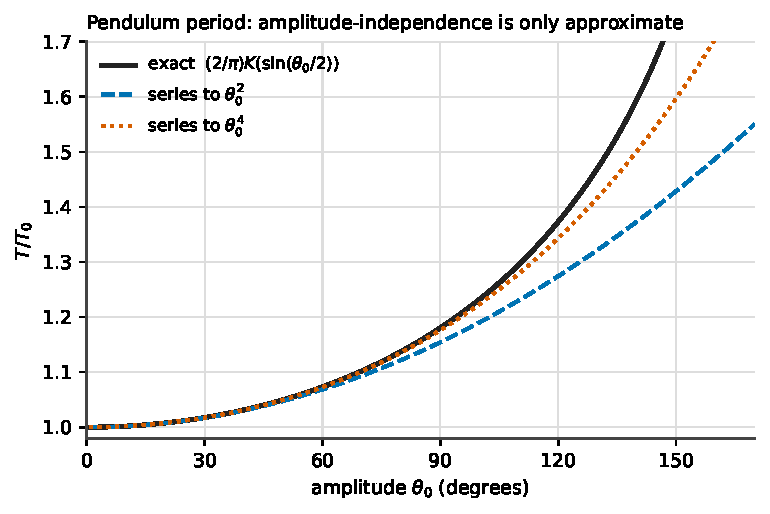
\includegraphics[width=0.62\textwidth]{figures/pendulum_series.pdf}
\caption{The registered small-angle chart against the exact libration period. The exact ratio $T/T_0=(2/\pi)K(\sin(\theta_0/2))$ (solid) is plotted with the two- and four-term small-amplitude series. All three agree to within a percent below roughly $40^\circ$, but the truncated charts diverge systematically as amplitude grows, so ``period independent of amplitude'' holds only inside the registered regime $|\theta_0|\ll 1$ and is refuted by finite-amplitude evidence outside it.}
\label{fig:pendulum-series}
\end{figure}

This distinction illustrates why context must be attached to claims. Define
\[
C_{\mathrm{exact}}=(\theta_0\in(0,\pi),\text{ideal pendulum},T(\theta_0)),
\]
and
\[
C_{\mathrm{small}}=(|\theta_0|\ll1,\text{linearized pendulum},T_0).
\]
The transition from the exact to the small-angle chart carries an approximation map and an error expansion. The two charts are coherent after that relation is registered. If the small-angle formula is asserted globally with its regime removed, it becomes a different claim and can be refuted by finite-amplitude evidence.

\subsection{Gravity, mass and context alignment}

The exact and approximate periods both scale as \(\sqrt{L/g}\). Changing from Earth to the Moon therefore changes the period through the local gravitational acceleration while preserving the structural form of the ideal model. By contrast, \(m\) cancels from the equation of motion. These facts have different epistemic roles:

\begin{itemize}[leftmargin=*]
\item ``period changes with \(g\)'' is a parameter-dependence statement;
\item ``period is independent of \(m\)'' is an ideal-model invariance;
\item ``period is independent of amplitude'' is only an approximation-level statement;
\item ``period depends on mass'' is incompatible with the registered ideal model unless some additional mass-dependent mechanism enters the context.
\end{itemize}

A real experiment can introduce such additional mechanisms. Air drag, bob geometry, string elasticity or pivot friction may correlate with mass. The correct response is not to force the observation into the ideal chart. It is to open or refine a context/mechanism fiber. The ideal invariant remains valid in its scope while the experimental chart records the extra physics.

\subsection{A typed epistemic trace}

Suppose the initial research state contains only the small-angle relation
\[
c_1:T\approx2\pi\sqrt{L/g}
\]
with a regime certificate \(|\theta_0|\ll1\). A finite-amplitude source or derivation adds
\[
c_2:T=4\sqrt{L/g}\,K(\sin(\theta_0/2)).
\]
The new object does not refute \(c_1\) because the registered transition identifies \(c_1\) as the leading approximation to \(c_2\). Instead, the atlas gains a representation/relation certificate and a more explicit scope boundary.

Now consider a candidate claim
\[
c_3:T\text{ increases with bob mass under the ideal model}.
\]
The Lagrangian derivation gives a structural falsifier: mass divides out of the Euler--Lagrange equation. A refuted \(c_3\) enters negative history rather than disappearing. That negative object can later prevent a language model from reintroducing the same unsupported dependency.

A fourth claim
\[
c_4:T_{\mathrm{Moon}}=T_{\mathrm{Earth}}
\]
looks superficially similar to mass invariance but fails after context alignment because the two charts have different \(g\). The contradiction is therefore not a generic ``same pendulum/different answer'' conflict; it is a parameter-context conflict localized to gravitational acceleration.

The sequence demonstrates why one evidence/support list is insufficient. The exact period derivation, the small-angle approximation, the ideal mass invariance, the Earth/Moon parameter change and a refuted mass-dependence claim occupy different typed roles. A structured answer can cite them separately instead of treating every retrieved source as interchangeable support.

\subsection{Geometric growth versus epistemic gain}

The pendulum also illustrates the metrology distinction used by the saturation rule. Let a registered target ask for a defensible account of period dependence. An initial transition from \(c_1\) to \(c_2\) can both add an atom and close a blocking epistemic cut: the target now has an amplitude-aware support path. Adding a second textual source that merely restates \(c_2\) may increase evidence bindings without adding an independent evidence root. Recording the refutation of \(c_3\) grows negative history without opening a new positive support path. Refining a fiber name changes representation without changing any of those epistemic coordinates.

A single ``knowledge volume'' number would mix these events. The non-compensatory growth vector instead records what changed. This is the same reason reproducibility reforms emphasize transparent evidence and independent checks rather than the mere abundance of published claims \cite{nosek2015,munafo2017}.

\subsection{What saturation would mean in the worked world}

For the pendulum target, a bounded saturation basis might declare: the ideal rigid pendulum plus specified perturbations; a fixed object-identity policy; a route family spanning mechanics texts, historical sources, exact nonlinear analyses, experimental deviations and adversarial alternative mechanisms; an evidence policy distinguishing derivation from experiment; and a freshness cutoff.

A round that discovers the elliptic-integral solution has \(\Delta D>0\). A round that discovers a previously omitted drag mechanism has \(\Delta M>0\) and likely \(\Delta A>0\). A round that finds an older source establishing the same function can have \(\Delta V>0\) because the novelty boundary changes even if no equation changes. A round that only rewrites the explanation more elegantly has zero substantive growth.

Only after the required route family is stable and repeated rounds produce
\[
\Delta_r=\mathbf0
\]
may the bounded target be called saturated. The certificate remains explicitly relative to the declared world. A new precision experiment or a newly relevant physical regime can reopen the state immediately.

\subsection{Discussion: what epistemic mechanics adds}

The framework should be read as a composition of established ideas with new governance boundaries, not as an attempt to replace the fields reviewed in Section~\ref{sec:foundations}. Belief revision already studies rational change \cite{agm1985,gardenfors1988}. Truth-maintenance systems already preserve justifications and alternative assumption environments \cite{doyle1979,dekleer1986}. Provenance systems already track lineage \cite{buneman2001,green2007,prov2013}. Sheaf and contextuality methods already formalize local-to-global obstruction \cite{abramsky2011,curry2014}. Global-workspace and blackboard theories already study bounded shared access \cite{hayesroth1985,nii1986,baars1988,dehaene2001}. Search and literature-discovery work already addresses vocabulary mismatch and remote connections \cite{furnas1987,swanson1986,garikaparthi2025}.

Epistemic mechanics contributes the joints between these components. A proposal is not a canonical update. Provenance is not authority. Coactivation is not compatibility. Pairwise compatibility is not global gluing. A compatibility complex is not automatically a lattice. Computational influence is not evidence. Search depth is not open-world coverage. Graph growth is not scientific progress. A flat graph is not saturation unless the discovery and review basis is stable. These boundaries are individually simple; their value is that they are represented in one executable state discipline rather than left as prose advice to an agent.

\subsection{Limitations and open fibers}

Several important coordinates remain open.

First, the paper is primarily formal and architectural. The software tests establish behavior of the reference mechanisms, not improved scientific discovery in the wild. Matched same-model evaluations are required to estimate whether the governance overhead improves correctness, calibration, novelty detection or research efficiency.

Second, OWMD's hidden-name benchmark is currently a regression contract. Prospective evaluation should freeze unseen mechanism identities before search, include multiple domains and score both recall and false-positive/transfer cost. The absence of such an experiment is why bounded discovery closure is not advertised as a learned universal discovery skill.

Third, the closure-system lattice theorem is conditional on a declared closure operator. The present compatibility code does not yet implement a universal scientific closure operator, and different scientific domains may require different closure semantics. Constructing such operators without smuggling unsupported inference into \(\cl\) is itself a research problem.

Fourth, independence remains a hard empirical and organizational property. Two evidence roots can share hidden upstream data; two internal reviewers can share the same model context; two search routes can call the same underlying index. The framework can require provenance fields and reject obvious aliasing, but genuine independence sometimes requires external experimental or reviewer separation.

Fifth, a fixed freshness cutoff is operational rather than metaphysical. Science continues after publication. Saturation therefore has a built-in expiration mechanism rather than a permanent completeness label.

\subsection{Conclusion}

Scientific research by language-model agents needs a mechanics of permission as much as a mechanics of generation. The framework developed here treats knowledge as typed external state, requires context before contradiction, separates compatibility from gluing, and separates both from authority. A transient workspace can make selected objects computationally global without making them scientifically true. OWMD can force discovery to leave the vocabulary that produced the current ontology without pretending that finite search exhausts the open world.

The long-form construction adds a final principle: research should continue while substantive epistemic growth continues. Under a finite declared expansion operator, this principle is an ordinary fixed-point computation. In open-world science it becomes a bounded certificate requiring stable routes, repeated zero-gain rounds, omission and nearest-work audits, closed blocking fibers and a current freshness horizon. The paper itself is governed by that rule. It is released not because a target page count has been reached, but because additional adversarial knowledge-acquisition passes cease to change the formal, evidential or novelty state under the declared basis.

That is the intended meaning of a saturated epistemic-mechanics lattice: not a claim that all knowledge has been accumulated, but a closed, auditable scientific state whose current derivations, evidence, conflicts, mechanisms and novelty boundaries have stabilized relative to an explicit research world.
